\chapter{Estado del arte}
En este capítulo se exponen los principales temas de interés para la realización de este trabajo, las investigaciones realizadas sobre la TPV y NF-TPV (termofotovoltaica de campo cercano) y el marco teórico sobre las diferentes maneras que se transmite el calor.

\section{Termo-fotovoltaica}
%%%%%%%%%%%%%%   THERMO PHOTOVOLTAICA       %%%%%%%%%%%%%
Un generador termo-fotovoltaico(TPV) se basa en la conversión de energía calorífica en energía eléctrica mediante el efecto fotovoltaico a través una célula termo-fotovoltaica sin requerir ninguna parte móvil, conocido este tipo de sistemas de generación como motores pasivos de calor, como se representa de una manera sencilla en la figura \ref{fig:TPV_Subsistema}.
\begin{figure}[H]
	\centering
	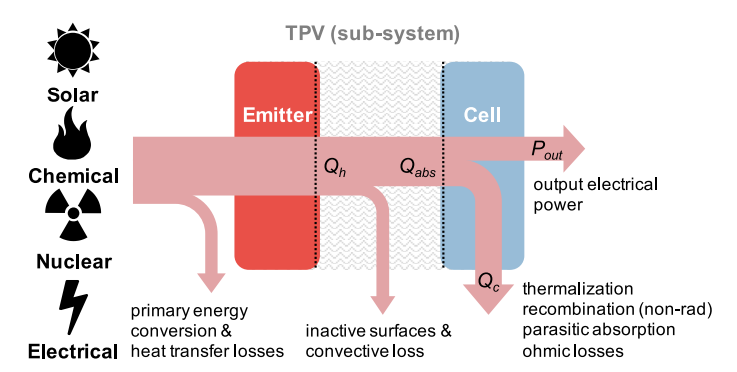
\includegraphics[width=0.7\textwidth]{figuras/TPV_Subsistema.png}
	\caption[Flujo de conversión de la energía térmica en energía eléctrica]{Flujo de conversión de la energía térmica en energía eléctrica. \textit{Figura obtenida de la referencia \cite{Present_Efficiencies_and_Future_Opportunities_in_Thermophotovoltaics}} }
	\label{fig:TPV_Subsistema}
	
\end{figure}
%\footnote{La figura \ref{fig:TPV_Subsistema} se obtuvo de la referencia \cite{Present_Efficiencies_and_Future_Opportunities_in_Thermophotovoltaics}}
El emisor se encuentra a una alta temperatura lo cual produce que se transmite el calor en forma de radiación, que al llegar a la célula es reflejada, transmitida o absorbida. La porción de radiación absorbida excita a los electrones produciendo un par electrón-hueco sí solo sí la energía del fotón absorbido es mayor que la energía del ancho de banda (\acrshort{ebg}) de la célula. Al conectar los terminales de la célula a una carga se produce una corriente que alimenta a la carga proporcional a la intensidad lumínica, aquellos fotones con energía menor a la \acrshort{ebg} son suprimidos o reflejados para disminuir el flujo de calor\cite{Present_Efficiencies_and_Future_Opportunities_in_Thermophotovoltaics}.\\\\
%%% INTERES EN LA TERMOFOTOVOLTAICA
La termofotovoltaica ha sido un campo de interés para aplicaciones militares, espaciales, generación de electricidad y recuperación de calor residual. Para la milicia de los Estados Unidos de América se han conducido varias investigaciones para la búsqueda de un generador eléctrico silencioso y portátil \cite{military_TPV}, cumpliéndose en 2004 40 años de investigación sin conseguirse potencias por encima de 500W \cite{military_TPV_40Years}. En aplicaciones espaciales es de interés por presentar beneficios en rendimiento para misiones cercanas al Sol y misiones en el espacio profundo porque los componentes más sensibles se encuentran resguardados de la dura radiación, siendo posible también el guardar energía en gravedad cero \cite{TPV_space_applications}. Para la recuperación de calor residual existe un gran interés porque la conversión de energía térmica a eléctrica es menor del 40\% en las plantas de generación de energía de combustibles fósiles convencionales, produciéndose una gran cantidad de pérdidas en forma de calor \cite{wasteHeat_TPV}.\\\\
%%% RESUMEN DE INVESTIGACIONES 
Todas estas áreas de interés han provocado un aumento de las investigaciones en los sistemas \acrshort{tpv}. Por ejemplo, la aplicación de capas finas en el emisor para aumentar la potencia radiada \cite{doi:Near_field_ThinFilm}, la aplicación de filtros  para la disminución de la cantidad de radiación no útil que llega a la célula \cite{multiLayerFilters}, la aplicación de capas traseras reflectantes (\acrshort{bsr}) para la recuperación de fotones \cite{thermoionic_TPV_NF}, la combinación con un \acrshort{tic} para aumentar la densidad de potencia y la eficiencia total del sistema generador \cite{thermoionic_TPV_NF,progress_Thermoionic_TPV}, y la disminución del espacio entre emisor y célula para aprovechar los efectos de la radiación de campo cercano\cite{thermoionic_TPV_NF,modelEfficiency_NF_TPV,nf_TPV_Pillars_SiO2}.\\\\
%\cite{thermoionic_TPV_NF,modelEfficiency_NF_TPV,nf_TPV_Pillars_SiO2,NearField_200nm}
%%%  OTRA INVESTIGACIÓN 
Las investigaciones no se han limitado a estudiar células TPV de una o varias uniones p-n, sino también la utilización de células \acrshort{tpv} interbandas en cascada (\acrshort{ictpv}) de \acrshort{bg} comprendidas entre 0.2 y 0.5 eV que resulta en una eficiente colección de portadores foto-generados, donde la eficiencia máxima ($\eta_{max}$) y la tensión de circuito abierto (\acrshort{voc}) es proporcional a el número de bandas hasta unos 0.691 V de \acrshort{voc} y uno 6.2\% $\eta_{max}$ \cite{MultiEstados_Capas_TPVs}.\\\\
%%%  BACK SURFACE REFLECTOR AND FILTERS
Aún quedan por estudiar muchos materiales y disposiciones del emisor y de la célula, algo de alta importancia es el estudio de filtros y \acrshort{bsr} porque aumentan la eficiencia y evitan que se acabe calentando innecesariamente la célula. Las \acrshort{bsr}, principalmente hechas de oro, reducen las pérdidas por absorción de la radiación de energía menor a la \acrshort{bg} porque reflejan la radiación que penetra la célula y la devuelve al emisor \cite{nTPV_Review}.\\\\
Habitualmente estas capas reflectantes se usan en las \acrshort{tpv} y \acrshort{tic}, como por ejemplo se usan en \cite{thermoionic_TPV_NF,modelEfficiency_NF_TPV,thermophotovoltaic_40}. Los filtros se utilizan para evitar la transmisión de radiación no deseada a la célula, consiguiéndose un aumento de la eficiencia del 45\% al 75\%. Los filtros pueden ser de una o múltiples capas, siendo afectada la eficiencia del conjunto según la rugosidad de las interfaces entre cada uno, obteniéndose mejores eficiencias al utilizar una menor cantidad de capas\cite{multiLayerFilters}.\\\\
%% Ahora va las investigaciones y poco a poco intercalando entre ellas
%%%  COMBINACION DE TPV CON TIC
La razón por la cual se combinan los \acrshort{tic} y las \acrshort{tpv} es para aprovechar tanto los electrones como los fotones radiados, aumentando la densidad de potencia de salida y mejorando el rendimiento de una \acrshort{tpv}. Si se disminuye la separación entre el emisor común y la célula por debajo de la micra se pasa a tener efectos de campo cercano, aumentando la potencia producida. En \cite{thermoionic_TPV_NF} se realiza un estudio teórico de una \acrshort{tpv} de campo cercano mejorado con termoiónico (\acrshort{nitpv}) con un emisor de grafito 1000 K y una célula \acrshort{pv} de $InAs$, que mejora el rendimiento y la densidad de potencia de una nTPV (TPV que aprovecha el efecto de campo cercano) de un $\sim$7\% de eficiencia y un $\sim 1 W/cm^{-2}$ de densidad de potencia a eficiencias superiores del 15\% y  densidad de potencia superiores a 10$Wm^{-2}$ (figura \ref{fig:PowerDensityVSEfficiency_nTiPV}), por el uso de una célula sin mallado, disminuyendo la resistencia en serie y las pérdidas por sombras, utilizando un BSR para reflectar los fotones de baja energía.\\
\begin{figure}[H]
	\centering
		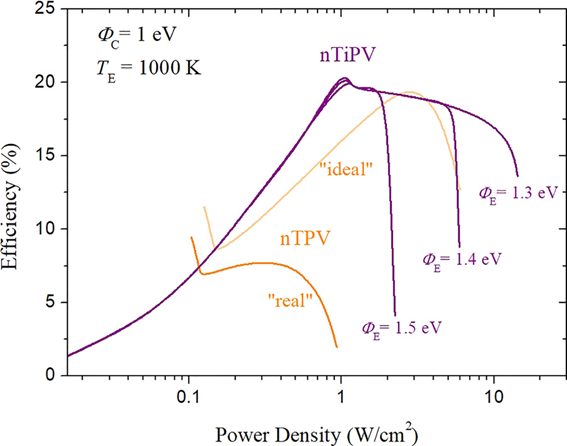
\includegraphics[height=7cm]{figuras/PowerDensityVSEfficiency_nTiPV.png}
	\caption[Relación entre densidad de potencia y eficiencia entre dispositivos nTPVs y nTiPVs]{Relación entre densidad de potencia y eficiencia entre dispositivos nTPVs y nTiPVs. \textit{Figura obtenida de la referencia \cite{thermoionic_TPV_NF}}}
	\label{fig:PowerDensityVSEfficiency_nTiPV}
\end{figure}
%%% CAMPO CERCANO
Los dispositivos \acrshort{tpv} que aprovechan el efecto de campo cercano se denotan como dispositivos \acrshort{nftpv}, \acrshort{nf-tpv} o \acrshort{ntpv}, los cuales son capaces de generar mayores potencias de salida que las \acrshort{tpv} por tener una mayor potencia de calor transmitida por radiación. Siendo un objetivo importante el aumento de la eficiencia, para así igualar a la actual de un 40\% \cite{thermophotovoltaic_40}. En \cite{modelEfficiency_NF_TPV} se modeló la eficiencia de un \acrshort{nf-tpv} basado en una célula de InAs a 300 K con emisor a 700 K y una distancia de separación de 200 nm, alcanzándose unas eficiencia del 17\% y notándose que a menores temperaturas y mayores distancias se obtiene una menor potencia de salida.\\\\
%%% DIFERENTES CERAMICAS
En \cite{differentEmitterCeramics} se evaluá teóricamente diferentes combinaciones de cerámicas para el emisor de una nTPV a 2000\textdegree C y célula a 400\textdegree C, observando los flujos espectrales de calor, la potencia total y el rendimiento, siendo la máxima potencia por metro cuadrado para el emisor de $B_4C$ con unos $7.45\cdot 10^4 \ Wm^{-2}$ pero solo con una eficiencia del 11.74\%, a diferencia del BeO con una potencia de $3.19\cdot 10^4 \ Wm^{-2}$ y un rendimiento del 24.69\%. Y se observa como el rendimiento disminuye al disminuir la separación entre emisor y célula para luego volver a aumentar.\\\\
%%% ECUACIONES
Dado que los costes de fabricación para el testeo pueden llegar a ser caros, se utilizan modelos matemáticos para simular, siendo uno muy útil el presentado en \cite{nfTPV_equations} que proporciona varias ecuaciones para calcular la potencia radiada para varios grosores de emisor y receptor de una sola capa cada uno, siendo el de mayor utilidad el de capa gruesa que proporciona de una manera sencilla el cálculo de la potencia en un rango de longitudes de onda conociendo la permitividad eléctrica compleja de los materiales.\\\\
%%% FRECUENCIA DE RESONANCIA Y CAPAS FINAS PARA AUMENTO DE ENERGIA
Una ventaja que presenta los \acrshort{nf-tpv} es el aumento de la potencia radiada para todas las longitudes de onda. Además, dependiendo de la combinación de los materiales utilizados, pueden aparecer frecuencias de resonancia (\gls{wres}) que producen un aumento significativo del flujo radiado a dicha frecuencia, pudiéndose aumentar la eficiencia de la \acrshort{nf-tpv} si se consigue que la \gls{wres} coincida con la \acrshort{bg} del semiconductor. Un ejemplo de esto se da en \cite{doi:Near_field_ThinFilm}, donde simulan un sistema \acrshort{ntpv} utilizando una lámina fina de carburo de silicio (\gls{sic}) y otra gruesa, obteniendo que al aumentar el grosor de la capa disminuye la potencia en la \gls{wres} pero aumenta para el resto de frecuencias, siendo a partir de los 100 nm de grosor la misma potencia radiativa que la lámina gruesa.\\\\
Para mantener las distancias de separación tan cortas en una \acrshort{ntpv} es necesario un mecanismo, siendo lo más sencillo el uso de pilares de algún material cerámico, por sus propiedades térmicas. Un ejemplo de esto se presenta en \cite{NearField200}, donde se estudia la transferencia de calor entre dos placas de Si separadas 200 nm por vacío y utilizando espaciadores de \gls{sio2} de 1 $\mu m$ de diámetro para mantener la distancia de separación. Obteniéndose que el coeficiente de transferencia de calor por radiación (\gls{hrad}) aumenta con la disminución de la separación entre emisor y célula, y la potencia radiada aumenta con la variación de la temperatura.\\\\
%%% RESISTENCIAS DE CONTACTO
También hay que tomar en cuenta que el coeficiente de transferencia de calor por conducción efectivo que se obtiene cuando se utilizan nano-espaciadores, depende principalmente de la resistencia térmica de contacto que se establezcan entre cada interfaz. En \cite{nf_TPV_Pillars_SiO2} se estudia la radiación por campo cercano entre dos placas de cuarzo con pilares piramidales truncados de $SiO_2$ que están depositados sobre el substrato inferior, descubriéndose que la resistencia de contacto (\acrshort{rc}) es mucho mayor que la geométrica del pilar. Por lo tanto, la \acrshort{rc} es de gran importancia para disminuir las pérdidas por conducción y así aumentar la eficiencia del sistema.
\section{Transmisión de calor}
Para una \acrshort{ntpv} el calor se propaga del emisor a la célula de tres formas distintas, por convección a través de un fluido, por radiación y por conducción a través de los nano-espaciadores.
\subsection{Convección}
La transmisión de calor por convección se produce por la conducción de la energía cuando el fluido entra en contacto con el sólido y luego el transporte de la energía mediante el movimiento del fluido, pudiendo ser natural o forzada. La diferencia entre la convección natural y la forzada es la fuente de movimiento del fluido, en la convección forzada el movimiento del fluido es producido por una fuente externa, como un ventilador o una bomba, en la convección natural el fluido se mueve por las diferencias en densidades por la variación de la temperatura de partes del fluido.\\

No se detalla más sobre este fenómeno de transporte de calor porque no se va a tener en cuenta a lo largo de este trabajo. Ya que supondremos que el sistema a estudiar se encuentra en una cámara al vació donde hay ausencia de fluido, en este caso, aire.
\subsection{Conducción}
La transmisión de calor por conducción se dá a través de uno o varios cuerpos, producido por la diferencia de temperatura entre las caras opuestas del conjunto o cuando dos o más objetos a diferentes temperaturas entran en contacto. De manera genérica la conducción térmica se modela como $P_{cond}={\bigtriangleup T}/{R} $, siendo $R$ la resistencia térmica del sistema.
Para un solo material, la resistencia térmica se modela como $R = l/{\left(A\cdot h\right)}$, donde $l$ es la longitud del material, $A$ es la superficie y $h$ es la conductividad térmica del material. Para varios materiales colocados en serie, es decir, el flujo de calor que los atraviesa es el mismo para todos, la resistencia de conducción se define como la sumatoria de todas las resistencias de cada material($R=\sum R_i$).\\

La superficie de contacto entre cada material se le conoce como interfaz, la cual en la realidad no es perfecta y provoca una caída de temperatura la cual se modela como una resistencia térmica llamada resistencia de contacto ($R_c$). La resistencia de contacto depende de muchos parámetros como la rugosidad de cada superficie, la presión, la temperatura, las conductividades térmicas de los materiales involucrados, los tipos de materiales, entre otros, esto provoca que sea muy difícil de obtener un modelo de la misma para una simulación.\\

En \cite{experimental_Rc_SS} se comparan la diferencia entre un modelo teórico y los resultados experimentales de la conductancia térmica de contacto respecto a la presión entre dos placas gruesas de varios materiales. Observándose que para dos aceros inoxidables 304 esta diferencia disminuye con el aumento de la presión, siendo la diferencia entre el modelo analítico y los resultados experimentales significativamente menor a partir de los 1 GPa de presión.

\subsection{Radiación}
La radiación es la transmisión de energía térmica en forma de ondas electromagnéticas o fotones a través del vacío o un medio material proporcional a la temperatura del cuerpo del emisor. Cuando las ondas electromagnéticas inciden sobre la superficie de un material parte de ella es absorbida, otra parte reflejada y el resto se transmite internamente en el material, variando las proporciones de dichas cantidades según el material y la longitud de onda de la radiación. Existe dos flujos de radiación conocidos, el flujo de propagación o campo lejano y el flujo evanescente o campo cercano que excede los valores predichos por la Ley de Planck del cuerpo negro.\\

\subsubsection{Radiación propagación o campo lejano}
La radiación de campo lejano cumple la ley de Planck sobre la emitancia monocromática de un cuerpo negro (${E_{\lambda}}^{bb}(T)$) (ecuación \ref{eq:ecuacionPlanck}), cuya integral cumple con la Ley de Stefan Boltzmann (ecuación \ref{eq:leyDeStefanBoltzmann}) y el valor máximo cumple con la Ley de Wien, $\lambda_{max}\cdot T=2.896\cdot 10^3 \mu m\cdot K$, donde la temperatura (T) está en grados Kelvin, $c_1$ es $3.743\cdot 10^8 \frac{W\mu m^4}{m^2}$ y $c_2$ es $1.4387\cdot 10^4 \mu mK$.

\begin{equation}
{E_\lambda}^{bb}\left( T \right) = \dfrac{c_1\cdot \lambda^{-5}}{e^{\frac{c_2}{\lambda \cdot T}}-1}
\label{eq:ecuacionPlanck}
\end{equation}
\begin{equation}
{E}^{bb}\left( T \right)=\sigma \cdot T^4 \qquad \Longleftrightarrow \qquad \sigma = 5.67\cdot 10^{-8} \dfrac{W}{m^2 K^4}
\label{eq:leyDeStefanBoltzmann}
\end{equation}

 Pero las ecuaciones anteriores solo aplica para la radiación total emitida pero no la transferida entre dos superficies, siendo el caso más sencillo el de dos superficies planas, paralelas entre sí y de área infinita o mucho mayor que la distancia que las separa, donde la transferencia de calor entre ambas superficies consideradas como cuerpos grises se puede modelar como:
\begin{equation}
\frac{\Phi}{S}=\frac{\sigma \left( T_1^4 -T_2^4 \right)}{1/\epsilon_1 +1/\epsilon_2 -1}
\label{eq:flujoCalorSuperficiesGrises}
\end{equation}
Donde $\epsilon_i$ es la emisividad monocromática, es decir, el cociente de la emisividad del cuerpo respecto a la del cuerpo negro, cuyo vaor es constante por ser considerados las superficies como cuerpos grises.\\\\
En este trabajo la radiación de propagación se resuelve de otra manera, que es el caso más sencillo de \cite{nfTPV_equations}, donde el emisor y el receptor son cuerpos planos y gruesos (figura \ref{fig:campoCercanoEquation1}) y la ecuación que modela el flujo de calor por frecuencia de un emisor (nº1) a un receptor (nº3) separados por el vacío (nº2) es:

\begin{equation}
q_{w,abs}^{prop}=\dfrac{\Theta \left( \omega,T_1 \right)}{4 \pi^2}\times \int^{k_\upsilon}_{0} k_\rho d k_\rho \sum_{\gamma=TE,TM}\dfrac{\left( 1- \left| r_{21}^\gamma \right|^2\right) \left( 1-  \left| r_{23}^\gamma \right|^2 \right)}{\left| 1- r_{21}^\gamma r_{23}^\gamma e^{2ik_{z2}d_{c}} \right|^2}
\label{eq:flujoPropNF}
\end{equation}
Donde $\Theta \left( \omega,T_i \right)$ es la energía media de un oscilador de Planck para una frecuencia y temperatura dada, $r_{i,j}^\gamma$ es el coeficiente de reflexión de Fresnel de la interfaz entre el cuerpo i y el cuerpo j en estado polarizado $\gamma$, TE son las ondas eléctricas transversales y TM son las ondas magnéticas transversales, i es la constante compleja $\sqrt{-1}$, $d_c$ es la separación entre las capas y $k_\rho$ es el vector de onda de la onda primaria \cite{nfTPV_fullEquations}.\\
\begin{figure}[H]
	\centering
		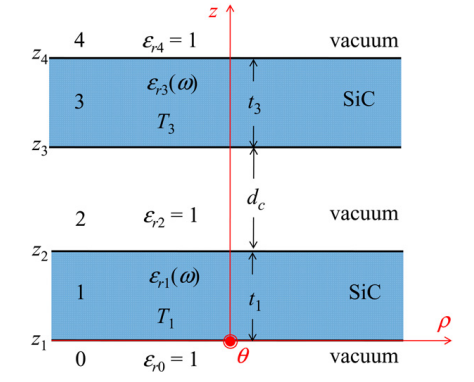
\includegraphics[height=7cm]{figuras/campoCercanoEquation1.png}
	\caption[Esquemático de la representación geométrica para el flujo entre dos cuerpos separados por vacío]{Esquemático de la representación geométrica para el flujo entre dos cuerpos separados por vacío. \textit{Fuente: \cite{nfTPV_equations}}}
	\label{fig:campoCercanoEquation1}
\end{figure}
La ecuación \ref{eq:flujoPropNF} es para dos placas gruesas separadas por un vacío y rodeadas por vacío, se obtiene de las ecuaciones presentadas en \cite{nfTPV_fullEquations}, donde se presenta las ecuaciones para la radiación de campo cercano de sistemas multicapa y un método numérico para solucionar las ecuaciones.

\subsubsection{Radiación evanescente o campo cercano}
La radiación evanescente a diferencia de la radiación de propagación, solo se transmite a distancias muy pequeñas porque decae exponencialmente con el aumento de la distancia de separación entre la fuente y el receptor. Esta potencia radiada puede llegar a superar a la potencia de un cuerpo negro por la ley de Planck.\\\\
Un modelo analítico es obtenido en \cite{nfTPV_fullEquations} para un sistema unidimensional de varias capas de diferentes grosores, temperaturas y materiales. Y también se introduce un algoritmo genérico para la implementación de las ecuaciones para simular.\\\\
En este trabajo se estudia un caso más sencillo, donde solo son dos capas gruesas separadas por vacío una distancia $d_c$ \cite{nfTPV_equations}, cuya ecuación que modela la potencia radiada por frecuencia de un emisor (nº1) a un receptor (nº3) separados por el vacío (nº2) es:

\begin{equation}
q_{\omega,abs}^{evan}=\dfrac{\Theta \left( \omega,T_1 \right)}{\pi^2}\times \int^{\infty}_{k_\upsilon}k_\rho d k_\rho e^{-2k_{z2}'' d_c} \sum_{\gamma=TE,TM} \dfrac{Im\left( r_{21}^\gamma \right)Im\left( r_{23}^\gamma \right)}{\left| 1- r_{21}^\gamma r_{23}^\gamma e^{2ik_{z2}d_{c}} \right|^2}
\label{eq:flujoEvasNF}
\end{equation}

Siendo $Im\left(r_{i,j}^\gamma \right)$ el término imaginario del coeficiente Fresnel de la interfaz entre el cuerpo \textit{i} y el cuerpo \textit{j} en estado polarizado $\gamma$. La componente $e^{-2k_{z2}'' d_c}$ representa de manera explícita la caída exponencial del flujo con la distancia de separación.\\\\
Una mejor representación del efecto de la radiación evanescente se puede observar en la figura \ref{fig:graficaDiff_dc_fullEqu}, donde a partir de cierta distancia de separación se supera el flujo de un cuerpo negro. Y se observa en la figura \ref{fig:graficaDiff_t_fullEqu} como a partir de las 100 $\mu m$ de grosor del emisor se puede considerar como una placa gruesa \cite{nfTPV_fullEquations}.

\begin{figure}[H]
\centering
\begin{subfigure}[b]{0.48\textwidth}
	\centering
		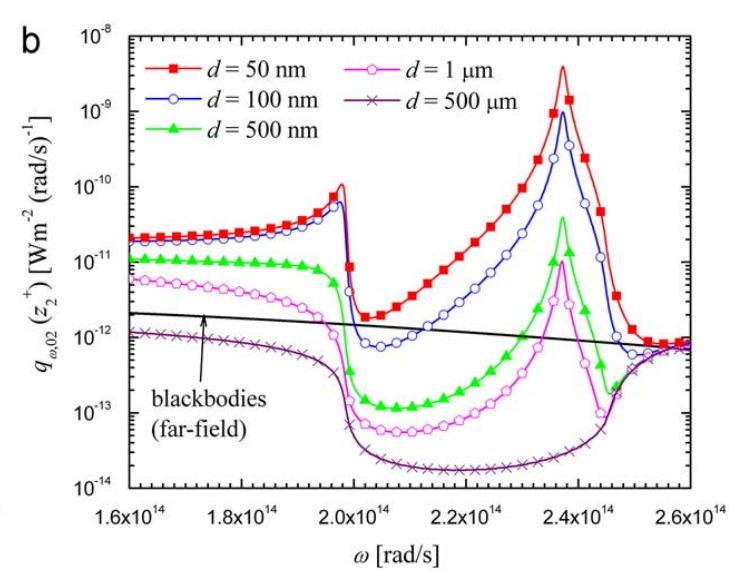
\includegraphics[width=\textwidth]{figuras/graficaDiff_dc_fullEqu.png}
		\caption{Flujo de radiación monocromática variando la distancia de separación d}
	\label{fig:graficaDiff_dc_fullEqu}
\end{subfigure}
\begin{subfigure}[b]{0.48\textwidth}
	\centering
		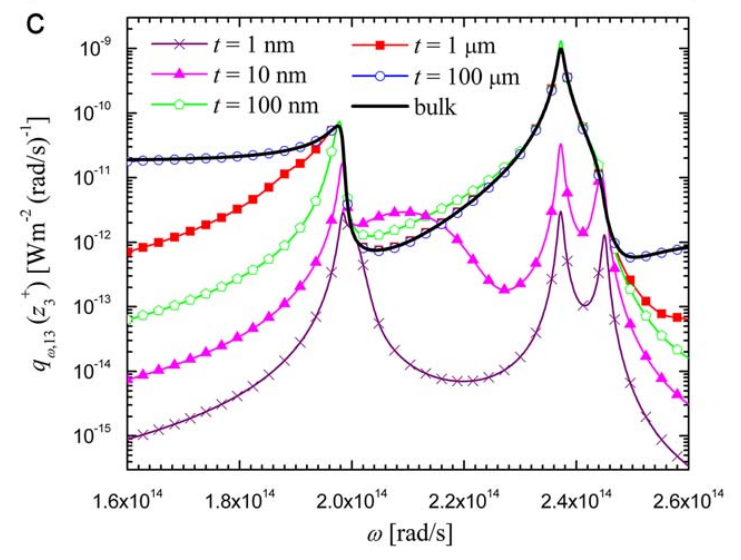
\includegraphics[width=\textwidth]{figuras/graficaDiff_t_fullEqu.png}
		\caption{Flujo de radiación monocromática variando el grosor (t) del emisor}
	\label{fig:graficaDiff_t_fullEqu}
\end{subfigure}
\caption[Flujos de radiación monocromática por variación de grosor de emisor y variación de distancia]{(\subref{fig:graficaDiff_dc_fullEqu}) Flujo de la radiación monocromática entre dos capas gruesas de cBN a 300 K y 0 K separadas por vació a una distancia d, y comparados con las predicciones de dos cuerpos negros en el régimen del campo lejano. (\subref{fig:graficaDiff_t_fullEqu})Flujo de la radiación monocromática entre un emisor de grosor (t) variable a 300 K y un receptor grueso a 0 K, ambos de cBN y separados por una distancia de 100 nm en el vacío. \textit{Ambas figuras han sido obtenidas de la referencia \cite{nfTPV_fullEquations}}}%
\label{fig:graficas_fullEqu}%
\end{figure}
También se puede observar en las figuras \ref{fig:graficas_fullEqu} \subref{fig:graficaDiff_dc_fullEqu} y \subref{fig:graficaDiff_t_fullEqu} el efecto de la \gls{wres} sobre la radiación espectral, aumentando considerablemente la potencia radiada a dicha frecuencia de $\sim 2.373\cdot 10^{14} \ rad/s$. Se puede observar como al disminuir el grosor del emisor se obtienen dos picos en vez de uno, pudiéndose considerarse casi monocromática alrededor de la \gls{wres}.\\\\
\vfill
